\section{SLAM}
When a robot is placed in an unknown environment, it needs to figure out where it is and how the world around it looks. For this SLAM is used, SLAM is short for Simultaneous Localization And Mapping. 
What want to achieve by using slam is to know the relative position of the robot to all seen landmarks. There is two main types of slam, online SLAM and full SLAM. online SLAM only keeps track of the relative position of the robot compared to all seen landmarks, while full SLAM keeps track of the current and all previous robot positions compared to all seen landmarks.
There are multiple SLAM algorithms, in this section, Graph SLAM will be explained shortly.

\subsection{Graph SLAM}
In the perfect world, when a robot moves, it will move exactly as intended. So if a robot is supposed to move 10 in the x direction, the new position will be $x_1 = x_0 + 10$ and $y_1 = y_0$. 
This, however is not the way it actually works. There will always be some motion noise. So instead of hitting the spot perfectly, the robot will hit the spot with some probability, which can be estimated by a Gaussian. So the new robot position will be constraint by:
\begin{equation}
f(x,y)=\frac{1}{\sqrt{2\pi\sigma^2}} \cdot e^(\frac{\frac{1}{2}(x_1-x_0-10)^2}{\sigma^2} \cdot \frac{1}{\sqrt{2\pi\sigma^2}} \cdot e^(\frac{\frac{1}{2}(y_1-y_0)^2}{\sigma^2}
\label{SLAM_eq01}
\end{equation}
This is pictured in figure \ref{SLAM_fig02}.
\begin{figure}[h!]
    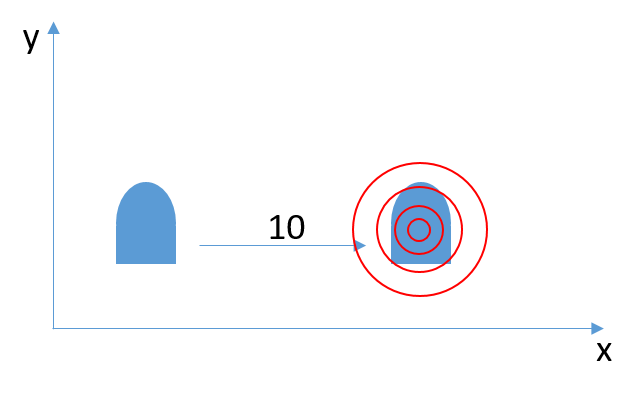
\includegraphics[scale=0.5]{billeder/GraphSLAM02.png}
    \caption{A robot in a non perfect world, moving 10 in the x direction. Noise is estimated as a Gaussian with mean $\mu = [10,0]$ and standard deviation $\sigma$.}
    \label{SLAM_fig02}
\end{figure}
What we want to do is to maximise the likelihood of the new position, given the previous position.
So what Graph SLAM does is defining the probabilities using a sequence of constraints like the one in equation \ref{SLAM_eq01}. 
If a robot moves in some space, each location is characterized by a vector that in a 2 dimensional world often is 3 dimensional (it will consist of a x-coordinate, y-coordinate and an angle). 
Graph SLAM then takes the following constraints: 
\begin{itemize}
\item \textit{Location Constraint}, which is just $x_0$.
\item \textit{Relative Motion Constraints}, which relates each robot pose to the previous robot pose. These can be seen as rubber bands.
\item \textit{Relative Measurement Constraints}, which relates each robot pose with the landmarks seen from that pose. These can also be seen as rubber bands.
\end{itemize}
Graph SLAM then relaxes the set of Relative Constraints to find the most likely configuration of a robot path along with the location of landmarks.
The way to do this is to use a quadratic matrix $\Omega$ and a vector $\xi$. $\Omega$ and $\xi$ consists of the addition of all constraints. Figure \ref{SLAM_fig04} shows an example of Graph SLAM using full SLAM. Every time a constrain is set it is added to the previous constrains. In the example, the constrains are added in the end for a better understanding of the individual steps.

\begin{figure}[H]
\centering
\begin{subfigure}{.5\textwidth}
  \centering
  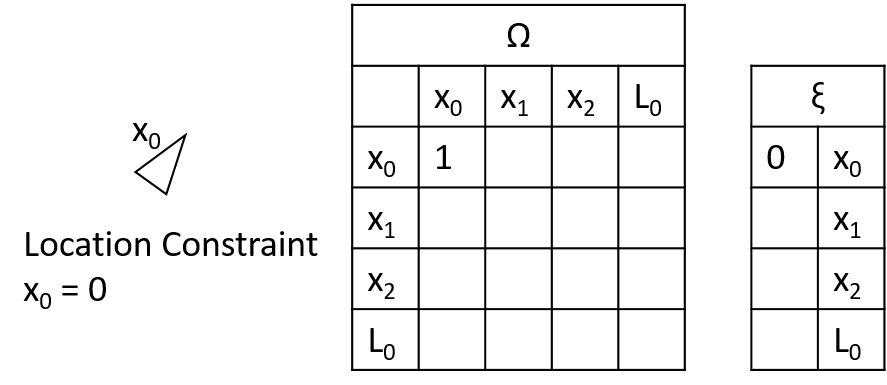
\includegraphics[width=.8\linewidth]{billeder/GraphSLAM04_1.png}
  \caption{Location Constrain}
  \label{SLAM_fig04:sub1}
\end{subfigure}%
\begin{subfigure}{.5\textwidth}
  \centering
  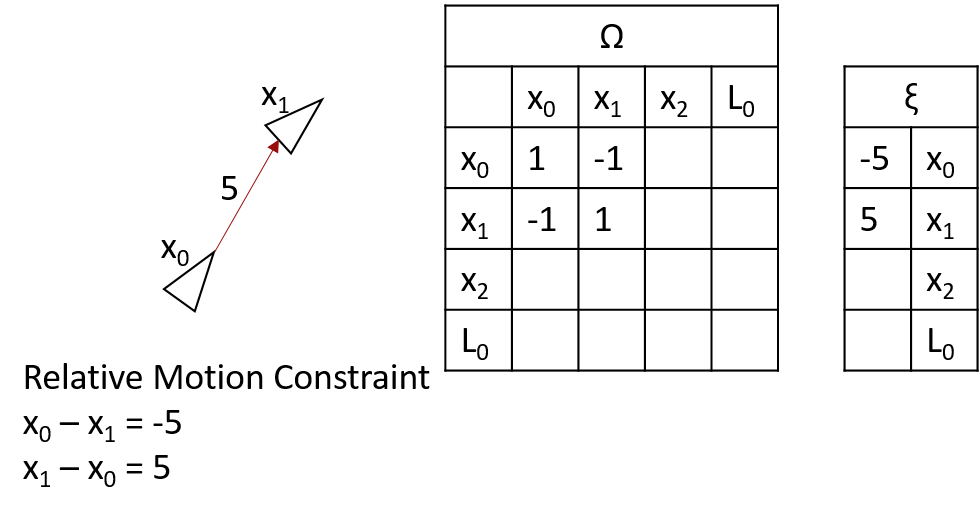
\includegraphics[width=.8\linewidth]{billeder/GraphSLAM04_2.png}
  \caption{Relative Motion Constrain from $x_0$ to $x_1$}
  \label{SLAM_fig04:sub2}
\end{subfigure}
\begin{subfigure}{.5\textwidth}
  \centering
  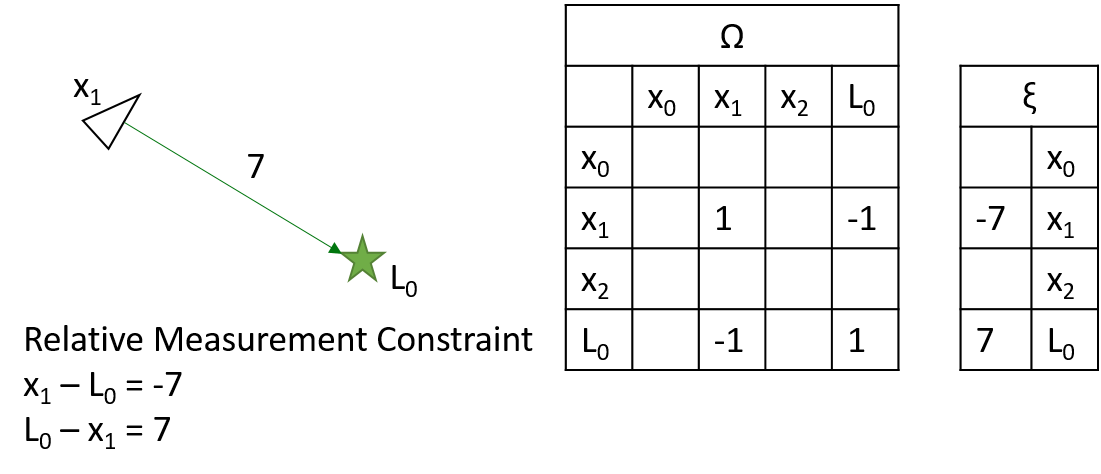
\includegraphics[width=.8\linewidth]{billeder/GraphSLAM04_3.png}
  \caption{Relative Measurement Constrain from $x_1$ to $L_0$}
  \label{SLAM_fig04:sub3}
\end{subfigure}%
\begin{subfigure}{.5\textwidth}
  \centering
  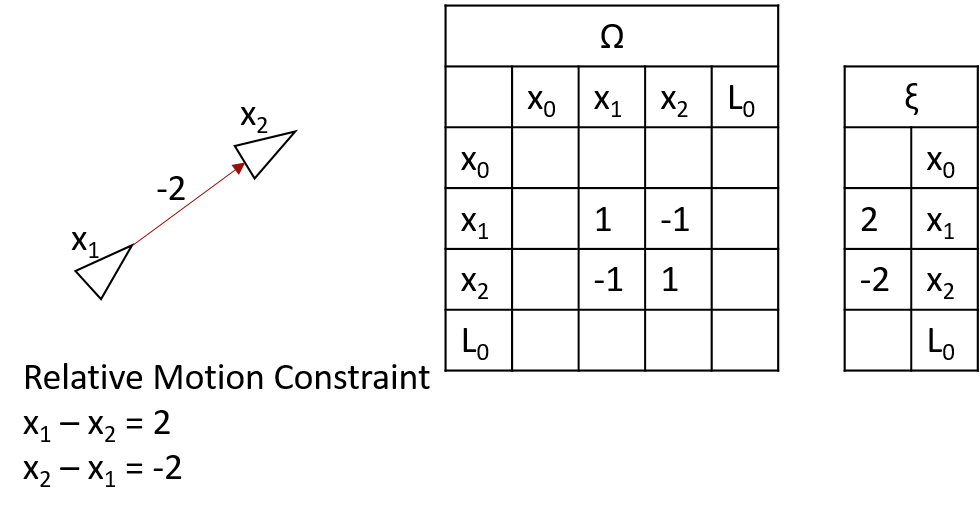
\includegraphics[width=.8\linewidth]{billeder/GraphSLAM04_4.png}
  \caption{Relative Motion Constrain from $x_1$ to $x_2$}
  \label{SLAM_fig04:sub4}
\end{subfigure}
\begin{subfigure}{.5\textwidth}
  \centering
  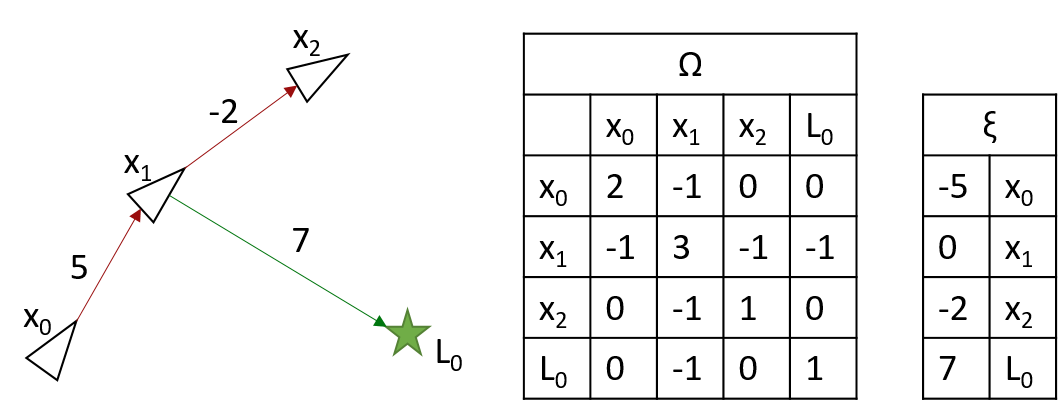
\includegraphics[width=.8\linewidth]{billeder/GraphSLAM04_5.png}
  \caption{The total Graph SLAM consists of the steps added together.}
  \label{SLAM_fig04:sub5}
\end{subfigure}
\caption{Graph SLAM illustrated.}
\label{SLAM_fig04}
\end{figure}

The most likely positions for the robot poses and the landmarks, $\mu$, are then found using equation \ref{SLAM_eq02}. 
\begin{equation}
\mu = \Omega^{-1} \cdot \xi
\label{SLAM_eq02}
\end{equation}

If noise is involved in the movements or measurements, this is handled by multiplying the constrains with $\frac{1}{\sigma}$, where $\sigma$ is the noise related to the constrain.

If the robot lives for a long time, the path taken will grow towards infinity. To avoid this, online SLAM can be used, but this will not be explained here.

%------------------------------------------------